\subsection{2017 Free-Response Questions}
Questions 1 and 2 are part of the same section and are allotted 30 minutes for completion with the aid of a graphing calculator.
Questions 3 through 6 are part of the same section and are allotted 1 hour for completion without the aid of a graphing calculator.

\begin{table}[H]
	\begin{center}
		\begin{tabular}{|c||c|c|c|c|}
			\hline
			$h$ (feet) & 0 & 2 & 5 & 10 \\
			\hline
			$A(h)$ (square feet) & 50.3 & 14.4 & 6.5 & 2.9 \\
			\hline
		\end{tabular}
	\end{center}
\end{table}

\begin{enumerate}
	
	\item A tank has a height of 10 feet.
		The are of the horizontal cross section of the tank at $h$ feet is given by the function $A$, where $A(h)$ is measured in square feet.
		The function $A$ is continuous and decreases as $h$ increases.
		Selected values for $h$ are given in the table above.
		\begin{enumerate}
			\item Use a left Riemann sum with three subintervals indicated by the data to approximate the volume of the tank.
				Indicate units of measure.
			\item Does the approximate in part (a) overestimate or underestimate the volume of the tank?
				Explain your reasoning.
			\item The area, in square feet, of the horizontal cross section at height $h$ feet is modeled by the function $f$ given by $f(h)=\frac{50.3}{e^{0.2h}+h}$.
				Based on this model, find the volume of the tank.
				Indicate units of measure.
			\item Water is pumped into the tank.
				When the height of the water is 5 feet, the height is increasing at a rate of 0.26 foot per minute.
				Using the model from part (c), find the rate at which the volume of water is changing with respect to time when the height of the water is 5 feet.
				Indicate units of measure.
		\end{enumerate}
	
	\begin{figure}[H]
		\label{2017_2}
		\centering
		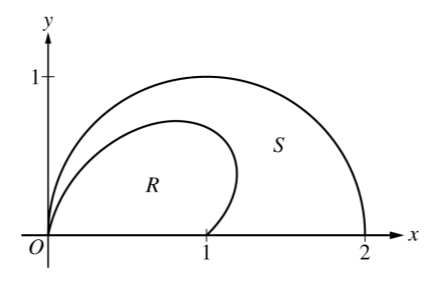
\includegraphics{./additional_materials/2017_2.png}
		\caption{\hyperref{https://apcentral.collegeboard.org/pdf/ap-calculus-bc-frq-2017.pdf}{}{}{AP Calculus BC 2017 Exam Free-Response Question 2}}
	\end{figure}

	\item The figure above show the polar curves $r=f(\theta)=1+\sin{\theta}\cos{(2\theta)}$ and $r=g(\theta)=2\cos{\theta}$ for $0 \leq \theta \leq \frac{\pi}{2}$.
		Let $R$ be the region in the first quadrant bounded by the curve $r=f(\theta)$ and the $x$-axis.
		Let $S$ be the region in the first quadrant bounded by the curve $r=f(\theta)$ the curve $r=g(\theta)$, and the $x$-axis.
		\begin{enumerate}
			\item Find the area of $R$.
			\item The ray $\theta = k$, where $0 < k < \frac{\pi}{2}$, divides $S$ into two regions of equal area.
				Write out, but do not solve, an equation involving one or more integrals whose solution gives the value of $k$.
			\item For each $\theta$, $0 \leq \theta \leq \frac{\pi}{2}$, let $w(\theta)$ be the distance between the points with polar coordinates $(f(\theta),\theta)$ and $(g(\theta),\theta)$.
				Write an expression for $w(\theta)$.
				Find $w_A$, the average value of $w(\theta)$ over the interval $0 \leq \theta \leq \frac{\pi}{2}$.
			\item Using the information given from part (c), find the value of $\theta$ for which $w(\theta)=w_A$.
				Is the function $w(\theta)$ increasing or decreasing at that value of $\theta$?
				Give a reason for your answer.
		\end{enumerate}
	
	\begin{figure}[H]
		\label{2017_3}
		\centering
		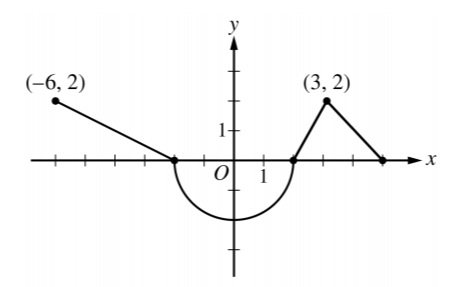
\includegraphics{./additional_materials/2017_3.png}
		\caption{\hyperref{https://apcentral.collegeboard.org/pdf/ap-calculus-bc-frq-2017.pdf}{}{}{AP Calculus BC 2017 Exam Free-Response Question 3, Graph of $f^\prime$}}
	\end{figure}
	
	\item The function $f$ is differentiable on the closed interval $[-6,5]$ and satisfies $f(-2)=7$.
		The graph of $f^\prime$, the derivative of $f$, consists of a semicircle and three line segments, as shown in the figure above.
		\begin{enumerate}
			\item Find the values of $f(-6)$ and $f(5)$.
			\item On what intervals is $f$ increasing?
				Justify your answer.
			\item Find the absolute minimum value of $f$ on the closed interval $[-6,5]$.
				Justify your answer.
			\item For each of $f^{\prime\prime}(-5)$ and $f^{\prime\prime}(3)$, find the value or explain why it doesn't exist.
		\end{enumerate}
	
	\item At time $t=0$, a boiled potato is taken from a pot on a stove and left to cool in a kitchen.
		The internal temperature of the potato is 91 degrees Celsius ($^\circ C$) at time $t=0$, and the internal temperature of the potato is greater than $27^\circ C$ for all time $t > 0$.
		The internal temperature of the potato at time $t$ minutes can be modeled by a function $H$ that satisfies the differential equation $\dd{H}{t} = -\frac{1}{4}(H-27)$, where $H(t)$ is measured in degrees Celsius and $H(0)=91$.
		\begin{enumerate}
			\item Write an equation for the line tangent to the graph of $H$ at $t=0$.
				Use this equation to approximate the internal temperature of the potato at time $t=3$.
			\item Use $\dd{^2H}{t^2}$ to determine whether your answer in part (a) is an underestimate or overestimate of the internal temperature of the potato at time $t=3$.
			\item For $t<10$, an alternate model for the internal temperature of the potato at time $t$ minutes is the function $G$ that satisfies the differential equation $\dd{G}{t} = -(G-27)^{2/3}$, where $G(t)$ is measured in degrees Celsius and $G(0)=91$.
				Based on this model, what is the internal temperature of the potato at time $t=3$?
		\end{enumerate}
	
	\item Let $f$ be the function defined by $f(x) = \frac{3}{2x^2-7x+5}$.
		\begin{enumerate}
			\item Find the slope of the tangent line of the graph of $f$ at $x=3$.
			\item Find the $x$-coordinate of each critical point of $f$ in the interval $1 < x < 2.5$.
				Classify each critical point as the location of a relative minimum, a relative maximum, or neither.
				Justify your answer.
			\item Using the identity that $\frac{3}{2x^2-7x+5} = \frac{2}{2x-5} - \frac{1}{x-1}$, evaluate $\int_{5}^{\infty}{f(x)\d{x}}$ or show that the integral diverges.
			\item Determine whether the series $\sum_{n=5}^{\infty}{\frac{3}{2n^2-7n+5}}$ converges or diverges.
				State the conditions of the test used for determining convergence or divergence.
		\end{enumerate}
	
	\begin{align*}
		f(0) &= 0 \\
		f^\prime(0) &= 1 \\
		f^{(n+1)}(0) &= -n\cdot f^{(n)}(0) \text{ for all } n \geq 1
	\end{align*}
	
	\item A function $f$ has derivatives of all order for $-1 < x < 1$.
		The derivatives of $f$ satisfy the conditions above.
		The Maclaurin Series for $f$ converges to $f(x)$ for $\abs{x} < 1$.
		\begin{enumerate}
			\item Show that the first four non-zero terms of the Maclaurin series for $f$ are $x - \frac{x^2}{2} + \frac{x^3}{3} - \frac{x^4}{4}$, and write the general term for the Maclaurin series for $f$.
			\item Determine whether the Maclaurin series described in part (a) converges absolutely, converges conditionally, or diverges at $x=1$.
				Explain your reasoning.
			\item Write the first four nonzero terms and the general term for the Maclaurin series for $g(x) = \int_{0}^{x}{f(t)\d{t}}$.
			\item Let $P_n\left(\frac{1}{2}\right)$ represent the $n$th degree Taylor polynomial for $g$ about $x=0$ and evaluated at $x=\frac{1}{2}$, where $g$ is the function defined in part (c).
				Use the alternating series error bound to show that
				\begin{equation*}
					\biggr\lvert P_4\left(\frac{1}{2}\right) - g\left(\frac{1}{2}\right) \biggr\rvert < \frac{1}{500}.
				\end{equation*}
		\end{enumerate}
	
\end{enumerate}